% !TEX TS-program = xelatex
% !TEX encoding = UTF-8 Unicode
% !Mode:: "TeX:UTF-8"
\documentclass{setting}
\usepackage{zh_CN-Adobefonts_external}
\usepackage{linespacing_fix} % disable extra space before next section
\usepackage{cite}
\usepackage{fancyhdr}
\definecolor{grey1}{rgb}{0.4, 0.4, 0.42}

\begin{document}
% \pagenumbering{gobble} % suppress displaying page number
\pagestyle{fancy}
\fancyhf{} % clear header and footer
\renewcommand{\headrulewidth}{0pt} % Remove header rule
\renewcommand{\footrulewidth}{0pt} % Remove footer rule
\lhead{} % Left header content (empty in this example)
\chead{} % Center header content (empty in this example)
\rhead{} % Right header content (empty in this example)

\lfoot{} % Left footer content (empty in this example)
\cfoot{} % Center footer content (empty in this example)
% \rfoot{} % Right footer content (empty in this example)
\rfoot{\color{grey1} \thepage/\pageref{LastPage}} % page number and last page

%%%% 利用tikz来定位学校Logo,这部分没有遵守College logo positioning
\begin{tikzpicture}[remember picture, overlay]
  \node[anchor = north west] at ($(current page.north west)+(1.45cm, -0.45cm)$) {
\includegraphics[width=2.5cm]{Picture/logo_KTH.png}};
\end{tikzpicture}
%%%% 利用tikz来定位照片
\begin{tikzpicture}[remember picture, overlay]
  \node[anchor = north east] at ($(current page.north east)+(-1.5cm, -0.2cm)$) {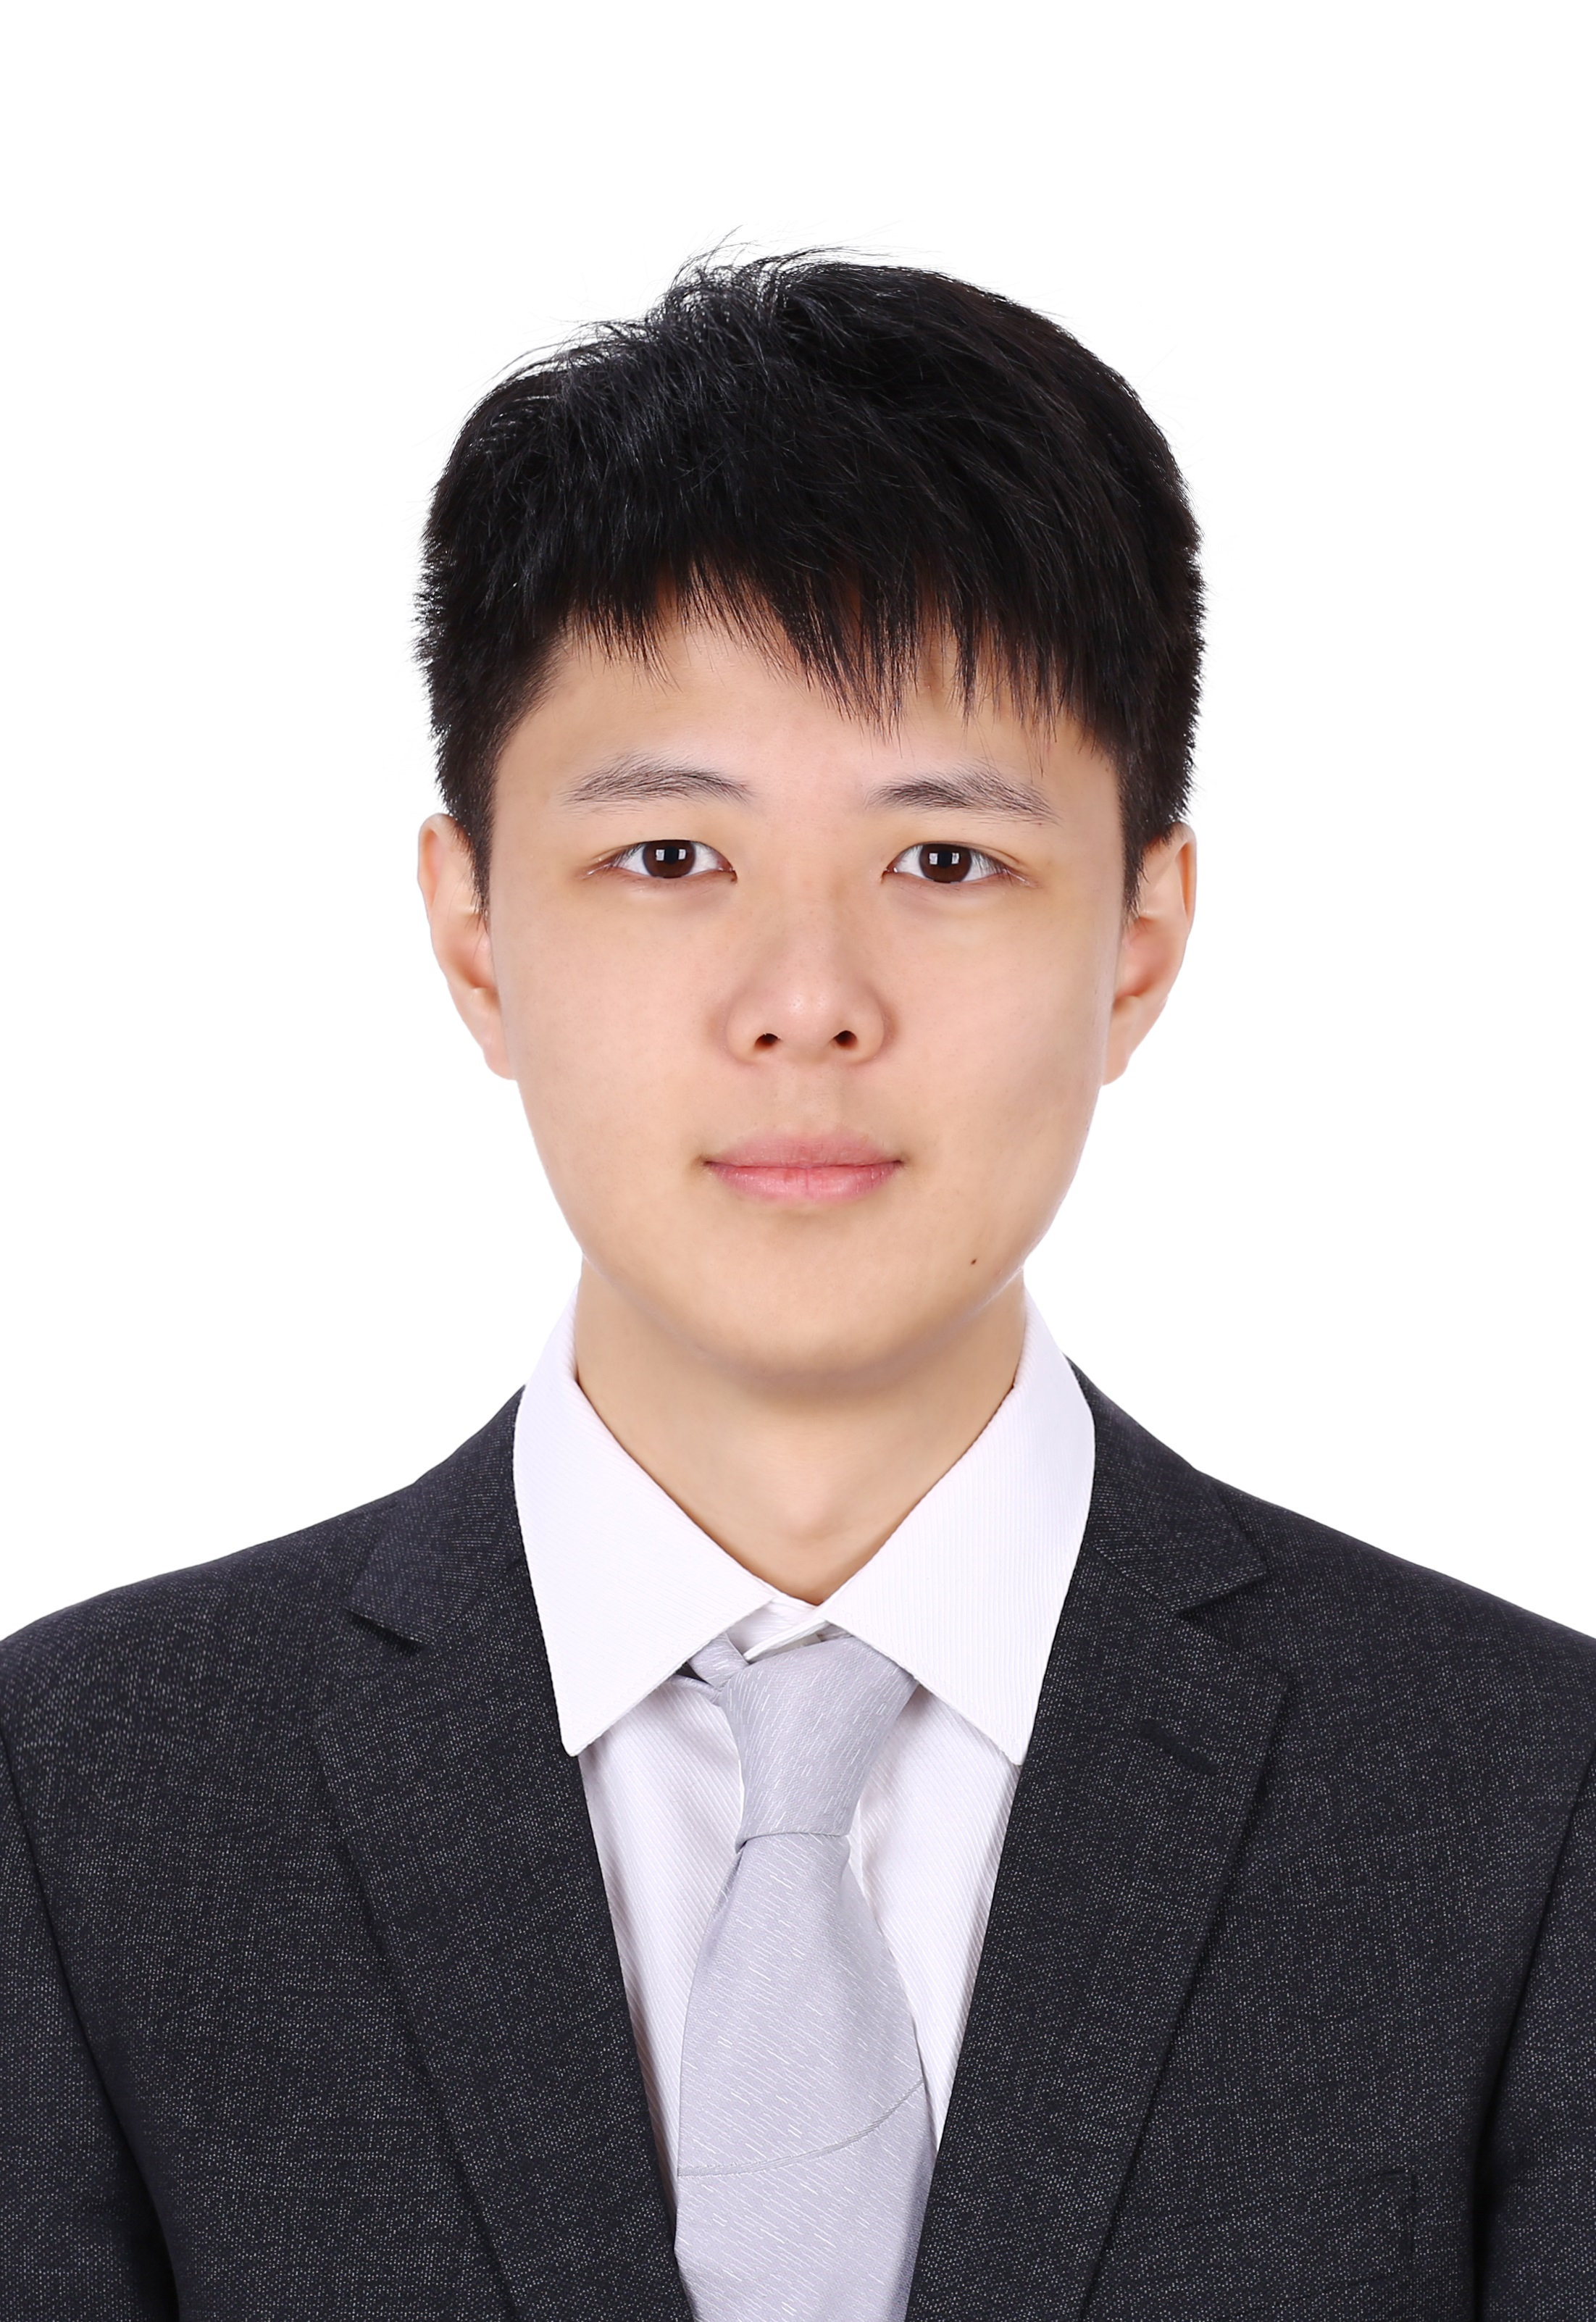
\includegraphics[height=3.5cm]{Picture/white.jpg}};
\end{tikzpicture}%

\name{牛雪芝}{}
\basicInfo{\phone{(+86)19382135251} \textperiodcentered\
    \email{xuezhiniu@163.com} \textperiodcentered\
    % \email{xuezhin@kth.se}
    \github[n7729697]{https://github.com/n7729697}
}

作为一名机电一体化专业毕业生,有很强的机械背景。我在设计和开发集成了机械、电子和软件组件的复杂系统方面拥有深厚的背景。在跨学科合作和领导团队实现项目里程碑方面有经验。熟练C/C++、Matlab、Python。精通使用 SolidWorks、AutoCAD、MATLAB、ROS 及其他软件进行设计和分析。具备硬件开发、3D 打印和 PCB 设计方面的专业知识。中英文流利。
\logosection{\faGraduationCap}{教育背景}
% \setcounter{}{}
\datedline{\textbf{瑞典乌普萨拉大学 Uppsala University}}{\dateRange{2024.01}{至今}}
\datedline{\tripleInfo{Ph.D. Embedded System}{\textit{博士在读}}{计算机系统系}}{瑞典乌普萨拉}
\datedline{\textbf{瑞典皇家理工学院 KTH Royal Institute of Technology}}{\dateRange{2021.09}{2023.12}}
\datedline{\tripleInfo{M.Sc. Mechatronics}{\textit{理学硕士}}{机电一体化和嵌入式控制系统系}}{瑞典斯德哥尔摩}
\begin{itemize}
  \item 硕士论文:基于模型的强化学习的软四足机器人的最优步态控制
\end{itemize}

\datedline{\textbf{香港城市大学 City University of Hong Kong}}{\dateRange{2017.09}{2021.07}}
\datedline{\tripleInfo{B.Eng. Mechanical Engineering}{\textit{工学学士}}{机械工程系}}{中国香港特别行政区}
\begin{itemize}
  \item 修读课程:控制理论基础、嵌入式系统、机器视觉、机器人学、信号及系统、C\texttt{++}、热力学、流体力学、材料力学、结构力学、CAD/CAM、现代控制理论、微机电系统(MEMS)、生产系统的运行管理等
\end{itemize}

\datedline{\textbf{新加坡国立大学 National University of Singapore}}{\dateRange{2020.01}{2020.06}}
\datedline{\tripleInfo{Mechanical Engineering}{\textit{交换生}}{设计与工程学院}}{新加坡}
% \begin{itemize}
%   \item 修读课程:微机电系统(MEMS)、生物材料、空气动力学、JAVA 
% \end{itemize}

% \logosection{\faSuitcase}{工作经历}

% \datedline{\textbf{血汗工厂}}{\dateRange{20xx.xx}{20xx.xx}}
% \datedline{建筑工程一线劳动者}{工地}

% 努力在率先实现社会主义现代化上走在前列

% \begin{itemize}
%   \item 
%   \begin{itemize}
%       \item 
%       \item 
%       \item 
%   \end{itemize}

% \end{itemize}

% \datedline{\textbf{远洋邮轮1号}}{\dateRange{20xx.xx}{20xx.xx}}

% \datedline{\tripleInfo{实习}{水手}{花式摸鱼工程师}}{精神家园}

% 负责策划麦哲伦五百年纪念活动, 坚持不忘初心
% \begin{itemize}
%   \item 精神荷兰人, 海上马车夫复兴者
%   \item 工人阶级的伟大代表 -- 不想当资本家的奴隶不是好工人
% \end{itemize}

\logosection{\faWrench}{项目经历}

\datedline{\textbf{基于模型的强化学习软四足机器人的最优步态控制} \href{https://urn.kb.se/resolve?urn=urn:nbn:se:kth:diva-339056}{\underline{Link}}}{\dateRange{2023.01}{2023.11}}
\datedline{\biInfo{\textit{学位论文}}{指导教师:\href{https://www.kth.se/profile/lfeng}{Prof. Lei Feng}}}{瑞典皇家理工学院}
\begin{itemize}
\footnotesize 
  \item \textbf{创新软件架构设计}:率先为新开发的利用3D打印制造的软式四足机器人设计并优化了软件架构,采用基于模型的强化学习来优化步态模式和运动
  \item \textbf{模拟和实验验证}:进行了大量的模拟和实验,利用数据驱动的洞察力,实现了比基准更优越的运动速度
  \item \textbf{多学科应用}:利用多学科知识,将基于模型的方法集成到软式四足机器人的软件架构和实际控制中,提高了强化学习效率,实现了最优步态控制
\end{itemize}

\datedline{\textbf{用于挤奶系统的电子真空可调截止阀} \href{https://urn.kb.se/resolve?urn=urn:nbn:se:kth:diva-324226}{\underline{Link}}}{\dateRange{2022.03}{2023.01}}
\datedline{\biInfo{\textit{项目实习}}{合作导师:\href{https://www.kth.se/profile/nilsjor}{Mr. Nils Jörgensen}}}{瑞典皇家理工学院 {\&} 瑞典利拉伐集团股份有限公司}
\begin{itemize}
\footnotesize 
  \item \textbf{机电系统集成设计}:与不同的工程师、研究人员和专家团队有效合作,成功设计并利用3D打印制造原型机,并应用于挤奶系统的真空度电子控制截止阀,提高了挤奶系统的稳定性,并且消除了系统中的真空度的下降
  \item \textbf{团队领导与研究}:作为团队负责人之一带头开发在Arduino上开发了阀门控制器和交互界面,实现了精确的无级调节,并集成了卡尔曼滤波器,以提高数据的准确性和可靠性
  \item \textbf{质量保证和合规性}:在整个设计和制造过程中确保严格的质量保证和符合行业标准,使用熔融沉积建模快速成型制造技术,确保原型制造的精度和效率
  \item \textbf{记录和报告}:由于在指导团队、项目规划以及确保项目执行方面的杰出领导能力和技术专长而受到表彰,熟练地记录实验程序、结果和分析,为项目文件和知识传播提供简明扼要的报告

\end{itemize}

% \datedline{\textbf{微机电系统(MEMS)执行器的设计制造}}{\dateRange{2022.10}{2023.01}}
% \datedline{\biInfo{\textit{项目课程}}{指导教师:\href{https://www.kth.se/profile/joachimo}{Prof. Joachim Oberhammer}}}{瑞典皇家理工学院}
% \begin{itemize}
% \footnotesize 
%   \item \textbf{质量控制}:领导了一个综合项目,重点设计和制造用于切换在光子网络光平面内路由电信信号的微机电系统(MEMS)执行器,在整个制造过程中实施严格的质量控制措施,确保 MEMS 执行器性能的可靠性和一致性
%   \item \textbf{仿真与优化}:利用COMSOL仿真分析致动器的电气和机械行为,优化其性能和精度
%   \item \textbf{微加工技术}:利用各种微细加工技术的熟练掌握,例如:光刻、干/湿蚀刻、PVD、CVD、电镀沉积、掺杂等技术,在实验室成功制造出了符合要求的微机电系统致动器(器件层厚度=30μm,最小特征尺寸=4μm,最小间隙=3μm),展示了将理论概念转化为实际应用的能力
%   % \item 领导了一个综合项目,重点设计和制造用于在光子网络光平面内路由电信信号的微机电系统(MEMS)执行器
%   % \item 利用COMSOL仿真分析致动器的电气和机械行为,优化其性能和精度
%   % \item 利用各种微细加工技术的熟练掌握,例如:光刻、干/湿蚀刻、PVD、CVD、电镀沉积、掺杂等技术,在实验室成功制造出了符合要求的微机电系统致动器(器件层厚度=30μm,最小特征尺寸=4μm,最小间隙=3μm)
%   % \item 展示了对微机电系统技术的深入理解,以及将理论概念转化为实际应用的能力
% \end{itemize}

\datedline{\textbf{单目自主飞行无人机}}{\dateRange{2022.01}{2022.06}}
\datedline{\biInfo{\textit{项目课程}}{指导教师:\href{https://www.kth.se/profile/patric/}{Prof. Patric Jensfelt}}}{瑞典皇家理工学院}
\begin{itemize}
\footnotesize
  \item \textbf{无人机导航与规划}:利用单目自主无人飞行器,搜索已知地图,以识别和辨认环境中的"入侵物体"(交通标志)
  \item \textbf{团队合作}:作为团队负责人之一研究基于Crazyflie 2.0和VM275T FPV摄像头的无人机定位、传感器融合和图像设别
  \item \textbf{算法设计与集成}:负责整体算法架构和无人机自主飞行的规划、定位和控制,在ROS上开发并集成了避障系统,使无人机在自主飞行时能够检测并有效躲避障碍物
  % \item 利用单目自主无人飞行器,搜索已知地图,以识别和辨认环境中的"入侵物体"(交通标志)
  % \item 作为团队负责人之一研究基于Crazyflie 2.0和VM275T FPV摄像头的无人机定位、传感器融合和图像设别
  % \item 负责整体算法架构和无人机自主飞行的规划、定位和控制,在ROS上开发并集成了避障系统,使无人机在自主飞行时能够检测并有效躲避障碍物
\end{itemize}

% \datedline{\textbf{无人车同时定位与地图构建(SLAM)}}{\dateRange{2022.01}{2022.06}}
% \datedline{\biInfo{\textit{项目课程}}{指导教师:\href{https://www.kth.se/profile/mjg?l=en}{Prof. Martin Edin Grimheden}}}{瑞典皇家理工学院}
% \begin{itemize}
% \footnotesize
%   \item \textbf{团队领导}:引领一个充满活力的五人团队,研究和开发基于Turtlebot3的无人车的运动轨迹规划和图像识别
%   \item \textbf{传感器数据融合}:融合了雷达和图像传感器的数据,增强了机器的感知能力,并确保了在不同场景下的稳健性能
%   \item \textbf{不断学习}:初步学习SLAM,设计并实施了综合算法架构,包括物体识别、精确定位、轨迹规划和控制,从而形成了一个完全自主的智能系统
%   % \item 利用C语言开发自动跟线行驶的引导车,在极限情况下,仅依靠红外线传感器完成路径搜索
%   % \item 开发基于LPCX13xx和红外线传感器的自动引导车的设计、控制和导航
%   % \item 负责整体算法架构和引导车的控制和导航
% \end{itemize}

\datedline{\textbf{液基气泡发电装置}}{\dateRange{2020.06}{2021.06}}
\datedline{\biInfo{\textit{毕业设计}}{指导教师:\href{https://www.cityu.edu.hk/stfprofile/zuanwang.htm}{Prof. WANG Zuankai 王钻开}}}{香港城市大学}
\begin{itemize}
\small 
  \item \textbf{理论研究}:开展对液态三电纳米发电机(TENG)的水基气泡发电的基础研究,所开发的实验发电设备能有效利用水基气泡发电,实现了每个气泡 3.4nW 的功率输出,具有较强的环境耐受度和可持续能源应用的潜力
  \item \textbf{概念实现}:利用自行设计的设备,设计并开发了一个定制实验装置,以验证液基 TENG 的概念和性能
  \item \textbf{项目管理}:展示了项目管理方面的专业知识,确保成功完成复杂的研究项目从开始到实际实施的整个过程
  % \item 开展对液态三电纳米发电机(TENG)的水基气泡发电的基础研究
  % \item 利用自行设计的设备,设计并开发了一个定制实验装置,以验证液基 TENG 的概念和性能
  % \item 所开发的发电装置实验发电设备能有效利用水基气泡发电,实现了每个气泡 3.4nW 的功率输出,具有较强的环境耐受度和可持续能源应用的潜力
\end{itemize}

% \datedline{\textbf{风力涡轮机叶片设计和原型制作}}{\dateRange{2021.01}{2021.05}}
% \datedline{\biInfo{\textit{课程设计}}{指导教师:\href{https://www.cityu.edu.hk/mne/people/academic-staff/prof-li-ky-lawrence}{LI K.Y.  Lawrence}}}{香港城市大学}
% \begin{itemize}
% \small 
%   \item \textbf{机械系统设计与优化}:熟练使用 SolidWorks 设计小型风力涡轮机叶片,确保最佳空气动力学和性能
%   \item \textbf{原型制造}:熟练掌握制造风力涡轮机叶片原型的 3D 打印技术,确保生产过程的精确性和准确性
%   \item \textbf{团队协作}:能有效地与团队成员合作,以实现项目目标并交付高质量的成果,参加课程竞赛,成功获得第二名
% \end{itemize}

% \datedline{\textbf{自动导引车AGV导航}}{\dateRange{2021.01}{2021.05}}
% \datedline{\biInfo{\textit{课程设计}}{指导教师:\href{https://www.cityu.edu.hk/mne/people/academic-staff/dr-liu-jun}{Prof. LIU Jun 刘军}}}{香港城市大学}
% \begin{itemize}
% \small 
%   \item \textbf{算法架构}:利用C语言开发出完全依靠红外传感器进行路径跟踪的引导车,在为AGV控制和导航设计综合算法、优化车辆性能和效率方面展示了专业知识
%   \item \textbf{嵌入式系统开发}:熟练使用 LPC13xx 微控制器和红外传感器设计、控制和导航自动制导车。领导开发了能够精确可靠导航的强大 AGV 系统
%   \item \textbf{跨学科协作}:与团队有效合作,成功领导AGV导航项目从执行到故障排除的整个过程,确保按时交付并达到项目里程碑
%   % \item 利用C语言开发自动跟线行驶的引导车,在极限情况下,仅依靠红外线传感器完成路径搜索
%   % \item 开发基于LPCX13xx和红外线传感器的自动引导车的设计、控制和导航
%   % \item 负责整体算法架构和引导车的控制和导航
% \end{itemize}

\datedline{\textbf{柔性电池的合成和制造}}{\dateRange{2019.04}{2020.01}}
\datedline{\biInfo{\textit{项目实习}}{指导教师:\href{https://www.cityu.edu.hk/mne/people/academic-staff/prof-zhang-kaili}{Prof. ZHANG Kaili 张开黎}}}{香港城市大学}
\begin{itemize}
\small 
  \item \textbf{理论研究}:作为研究助理对金属氢氧化物进行研究,利用种子辅助合成法制备柔性电池
  \item \textbf{实验设计与分析}:参与柔性电池测试、数据分析和结果总结等实验,所参与实验的新型合成方法和所设计的组装模组皆已申请发明专利
  \item \textbf{行业合作}:尝试与工业界合作,将柔性电池技术从概念推向市场,参与市场调研和产品测试
  % \item 对金属氢氧化物进行研究,利用种子辅助合成法制备的柔性电池进行实验,分析数据,并总结实验结果
  % \item 所参与实验的新型合成方法和所设计的组装模组皆已申请发明专利
\end{itemize}

% \datedline{\textbf{骨骼愈合的监测和预测}}{\dateRange{2018.09}{2019.01}}
% \datedline{\biInfo{\textit{项目实习}}{指导教师:\href{https://ece.hkust.edu.hk/eeyajing}{申亚京 SHEN, Yajing}}}{香港城市大学}
% \begin{itemize}
% \small
%   \item \textbf{文献综述与分析}:精通进行全面的文献综述,以收集相关信息,研究多传感器生物体内的协同探测
%   \item \textbf{数据收集和分析}:收集和分析实验数据,解释实验结果,以深入了解骨愈合的进展情况,并预测可能出现的结果
% \end{itemize}

% \newpage
\logosection{\faCogs}{专业技能}
\begin{itemize}[parsep=0.5ex]
  \item 编程语言: C/C\texttt{++} = Matlab = Python > \textsc{java} $\gg$ \texttt{C\#}
  \item 软件: 熟练使用SolidWorks, AutoCAD, MATLAB, Endnote, Zotero, LS-DYNA, ANSYS, COMSOL, Ubuntu, EAGLE, ROS, \LaTeX,easyEDA, Simplify3D, UltiMaker Cura, Adobe Premiere Pro, OriginLab, Adobe Illustrator, SPSS, MS Office等软件,并能快速学习任何已知软件
  \item 硬件:STM32F1/F3、NXP LPC13xx、Arduino/树莓派、3D打印(FDM、SLA)、激光切割、车床和铣床、PCB裸板制作(LPKF)、BNO055 IMU、PCB焊接与测试、电化学测试平台(辰华、新威尔、蓝电)、透射电子显微镜TEM(JEOL JEM-2100)/扫描电子显微镜SEM(FEI Quanta 450)
  \item 语言: 中文 - 母语,英语 - 熟练,德语 - 日常读写,瑞典语 - 初学
\end{itemize}

\logosection{\faInstitution}{公开成果及获奖}
% \datedline{\textit{发明专利(实质审查),CN 113675454 A,“一种小型柔性电池组装模具”}}{2020.6}
\datedline{\biInfo{\textit{才艺发展奖学金}}{香港特别行政区政府奖学金}}{2020.6}
\datedline{\textit{发明专利(实质审查),CN 14180645 A,“多元金属氢氧化物及其制备方法与应用”}}{2020.2}
\datedline{\biInfo{\textit{教育部第十六届“挑战杯”大学生课外学术科技作品竞赛}}{国赛二等奖}{队长}}{2019.11}
\datedline{\biInfo{\textit{教育部第五届“互联网 +”大学生创新创业大赛}}{国赛银奖}{核心成员}}{2019.10}
\datedline{\biInfo{\textit{第八届“赢在广州”暨粤港澳大湾区大学生创业大赛}}{银奖}{核心成员}}{2019.7}
\datedline{\biInfo{\textit{第五届香港大学生创新创业大赛}}{科技创新组第二名}{核心成员}}{2019.4}

% \logosection{\faBell}{社会服务}
% \datedline{\biInfo{\textbf{共融号-香港文化考察之旅}}{UNLEASH FOUNDATION }{志愿者}}{2018.1}
% \textit{获得聘志发展基金资助,以志愿服务的形式,促进内地学生来港的交流与融入。团队8人服务内地学生200人次,个人服务时长超过100小时。}
% \datedline{\biInfo{\textbf{E-buddy}}{TECC (Technology \& Education: Connecting Cultures) 香港分处}{项目负责人}}{\dateRange{2017.09}{2018.06}}
% \textit{以志愿服务的形式,通过线上连线的方式,于每周固定时间对留守儿童、孤儿、罕见病儿童、缺乏教育资源地区学生的课外拓展和课程答疑,并组织暑期回访,服务对象达195人次,团队服务时长超过500小时}
% \datedline{\biInfo{\textbf{运营部}}{TECC (Technology \& Education: Connecting Cultures) 香港分处}{核心成员}}{\dateRange{2017.09}{2019.01}}
% \textit{协调组织运作,进行活动组织策划,组织开展了多项活动,包括NLTP NPO领导力培训、TSI暑期教师学院、YAMP中华民族传承人培养计划等,组织参与人次达到500,参与时长超过200小时}

\logosection{\faBell}{兴趣爱好}
\datedline{\biInfo{Edmond Ko教授杯宿间足球赛}{汇丰业昕堂(Hall 2)}{冠军}}{2019.04}
\datedline{\biInfo{随州市中小学足球比赛}{高中组}{冠军}}{2016.06}
\datedline{\biInfo{全国中学生生物学联赛}{湖北省}{省二等奖}}{2016.04}
\par 擅长烹饪,具有6年烹饪经验,掌握中西菜系的各式家常菜、甜点、面食
\par 喜好阅读,已读超过300本各类小说
\label{LastPage}

%%%% 如果多页简历,可以手动在适当位置插入 \newpage 或者 \clearpage 开始新一页

% \begin{tikzpicture}[remember picture, overlay] 
  \node[anchor = south,fill=KTHBlue,draw=none,minimum width=\paperwidth,minimum height=1.5em,align=center,font=\footnotesize,text=white] at ($(current page.south)$) {\faLinkedinSquare \ https://www.linkedin.com/in/username \qquad \faGithub \ https://github.com/username \qquad \faRssSquare \ http://blog.yours.me};
\end{tikzpicture}

\end{document}
